\documentclass[11pt,a4paper]{article}

\usepackage[utf8]{inputenc}
\usepackage[T1]{fontenc}
\usepackage[english]{babel}
\usepackage{lmodern}
\usepackage{microtype}
\usepackage{geometry}
\geometry{margin=1in}
\usepackage{setspace}
\onehalfspacing
\usepackage{hyperref}
\hypersetup{colorlinks=true, linkcolor=black, citecolor=black, urlcolor=blue}
\usepackage{amsmath,amssymb}
\usepackage{booktabs}
\usepackage{array}
\usepackage{longtable}
\usepackage{enumitem}
\usepackage{tikz}
\usetikzlibrary{arrows.meta,positioning,fit,shapes.geometric,calc}
\usepackage{caption}
\usepackage[backend=biber,style=authoryear,natbib=true,maxcitenames=2,maxbibnames=6]{biblatex}
\addbibresource{references.bib}
\usepackage{xcolor}
\usepackage{fancyhdr}
\usepackage{titlesec}

\setlength{\headheight}{14pt}
\pagestyle{fancy}
\fancyhf{}
\lhead{Hyperautomation, Work Fragmentation, and Systemic Capability}
\rhead{Draft memo}
\cfoot{\thepage}

\titleformat{\section}{\large\bfseries}{\thesection}{0.6em}{}
\titleformat{\subsection}{\normalsize\bfseries}{\thesubsection}{0.6em}{}

\newcommand{\memo}[1]{\vspace{0.5em}\noindent\fbox{\begin{minipage}{0.95\linewidth}\textbf{Memo note.} #1\end{minipage}}\vspace{0.5em}}

\title{\textbf{From Hyperautomation to Systemic Engineering Capability}\\
\large A Reflective Research Memo on Work Fragmentation, Offshoring, Generative AI, and Latin American Innovation Capacity}
\author{Guillaume Harbonnier\\
\small Engineering / Quality Engineering / Systems Thinking Memo\\
\small Personal draft for LinkedIn appendix -- not an employer position}
\date{May 2026}

\begin{document}
\maketitle

\begin{abstract}
This research memo develops a personal but evidence-informed argument about hyperautomation, offshoring, and the future of engineering work. The central claim is not that generative AI will destroy ``work'' in general, but that it will disproportionately expose work that has been fragmented, routinized, and disconnected from system-level understanding. This is especially relevant for delivery models shaped by offshore cost arbitrage, where tasks may be optimized locally while systemic competence remains underdeveloped. Drawing on sociotechnical systems theory, organizational learning, the exploration/exploitation literature, and historical innovation environments such as Bell Labs, Xerox PARC, Embraer, and Intel Costa Rica, the memo argues for a shift from narrowly specialized execution to connected specialization: deep expertise combined with broader system, risk, business, and innovation awareness. The Latin American context is treated not as a deficit space but as a region with strong engineering talent and underused innovation potential, constrained by relatively low R\&D intensity, brain drain, and uneven university-industry collaboration. The memo closes with a leadership model based on gradual capability building: encouraging BA-QA cross-learning, QA-to-architecture exposure, prototyping, automation literacy, domain knowledge in biometrics and identity, and a culture of ``showing by doing.''
\end{abstract}

\noindent\textbf{Keywords:} hyperautomation; generative AI; offshoring; work fragmentation; quality engineering; systems thinking; Latin America; sociotechnical systems; organizational learning; Bell Labs; Embraer; leadership.

\section{Introduction: the uncomfortable question behind hyperautomation}
The public debate around generative AI often starts from an emotionally charged question: will AI destroy jobs? In my operational experience, the more accurate question is different: which kinds of work have we already made easy to automate by fragmenting them into narrow, repeatable, locally optimized tasks?

The distinction matters. A task that is isolated, repeatable, standardized, and detached from systemic context is not only easier to offshore. It is also easier to model, orchestrate, and eventually automate. This is not a moral judgment against specialization. Specialization has enabled industrial quality, scale, repeatability, and professional excellence. But specialization becomes risky when it turns into cognitive enclosure: people execute their fragment without seeing the system, the user, the risk, the economics, or the political and social consequences of failure.

In many organizations, the vocabulary itself reveals the drift. When a large IT service is called a ``software factory,'' the intention is usually positive: industrialization, delivery discipline, reusable components, and predictable output. Yet the metaphor also creates a cultural precedent. It suggests that software production can be treated as an assembly process. Once work is imagined as factory work, it is easier to segment, benchmark, outsource, and replace. The risk is not only technical. It is cultural.

\memo{This text is deliberately written as a hybrid: part research memo, part personal leadership reflection. It proposes conceptual interpretations grounded in operational experience and selected literature; it is not a statistically validated causal model. Operational examples are illustrative composites inspired by real-world system dynamics and do not describe any identifiable individual, client, production environment, or operational incident. I am trying to formalize what I have observed while managing BA/QA/QE teams in complex identity and biometric systems in Latin America.}


\section{Field observation: quality control, documents, and irreversible errors}
Consider a concrete example from secure document production and quality control. Human operators perform tasks such as visual inspection of documents, tactile verification of physical security features, chip reading, lot preparation, and transfer to dispatch. Technically, many of these steps could be automated through industrial vision, trusted cameras, robotics, biometric verification, and AI-based anomaly detection.

Yet the decision is not simply whether automation is possible. It is whether automation preserves the right balance between value, risk, reversibility, and trust -- and crucially, whether it changes the shape of failure.

Take an illustrative case that seems trivial until it is not: an applicant whose facial features are statistically unusual with respect to the reference data used by a model. An automated biometric or document-consistency check may pass this without hesitation. Not because it made a loud, detectable error. Because it made no error at all, by its own logic. The anomaly was simply outside, or insufficiently represented within, the distribution the model was optimized on. This is a \emph{silent false negative}: no alert, no flag, no friction. The document proceeds.

A human operator, fatigued or distracted, might also miss it. This is an honest concession. But the failure modes are structurally different. Human error tends to carry friction: a moment of doubt, a second look, a question to a colleague, a feeling that something is off. That friction is not inefficiency. It is a weak signal worth preserving. AI error at scale carries none of that friction. It can be fast, silent, and uniform -- which means it can be massively wrong before anyone notices.

This reframes the automation tradeoff. The question is not whether humans are more reliable than machines in the average case. Often they are not. The question is: whose errors do we prefer, and why? An error rate of 0.1\% applied uniformly across ten million documents is a different kind of risk than an error rate of 1\% distributed across human operators who sometimes catch each other's mistakes. Volume, silence, and the absence of natural correction mechanisms change the arithmetic entirely.

Automation does not eliminate error. It transforms its texture.

\begin{table}[h!]
\centering
\small
\begin{tabular}{p{0.24\linewidth}p{0.32\linewidth}p{0.32\linewidth}}
\toprule
\textbf{Dimension} & \textbf{Human failure mode} & \textbf{AI failure mode} \\
\midrule
Detection & Often noisy: doubt, second looks, peer questions & Often silent: no alert if the anomaly is outside the model's learned frame \\
Scale & Usually local and varied & Potentially uniform and scalable \\
Correction & Can benefit from informal escalation and redundancy & Often requires monitoring, retraining, rule updates, or process redesign \\
Trust impact & May remain contained if caught inside the process & Can become a public trust event if it propagates silently \\
\bottomrule
\end{tabular}
\caption{A simplified comparison of human and AI failure textures. The point is not that one is always safer, but that their failure modes differ structurally.}
\end{table}

In a document issuance process, a wrong portrait, an incorrect citizen representation, or a duplicated first name may be expensive to fix after printing, but still manageable if detected internally. Traceability and security can be preserved. If the same error reaches distributed lots, the cost rises sharply. If the document is delivered automatically to a citizen, the failure becomes public and potentially scandalous.

\begin{quote}
A bug inside the process is a cost. A bug visible to the citizen is a trust event. And a bug that scales silently before anyone notices is a crisis.
\end{quote}

The problem becomes sharper in first issuance. In identity systems, first issuance often relies on data that is effectively one-shot: difficult to replay, difficult to verify later, and potentially foundational for downstream records. Automating such a step without modelling irreversibility is not automation strategy. It is risk transfer.

\begin{figure}[h!]
\centering
\resizebox{\linewidth}{!}{%
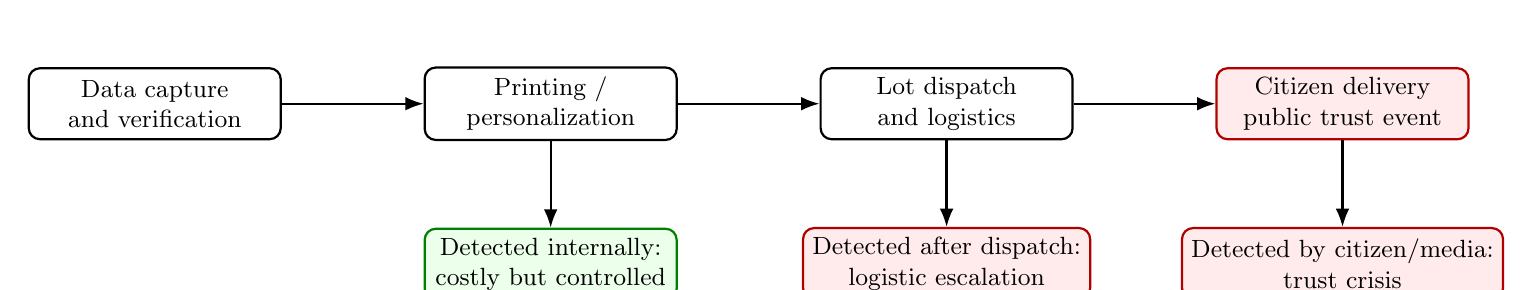
\begin{tikzpicture}[node distance=1.8cm, every node/.style={font=\small}, box/.style={rectangle, rounded corners, draw=black, thick, align=center, minimum width=3.2cm, minimum height=0.9cm}, risk/.style={rectangle, rounded corners, draw=red!70!black, thick, align=center, minimum width=3.2cm, minimum height=0.9cm, fill=red!8}, ok/.style={rectangle, rounded corners, draw=green!50!black, thick, align=center, minimum width=3.2cm, minimum height=0.9cm, fill=green!8}, arrow/.style={-{Latex}, thick}]
\node[box] (capture) {Data capture\\and verification};
\node[box, right=of capture] (production) {Printing /\\personalization};
\node[box, right=of production] (dispatch) {Lot dispatch\\and logistics};
\node[risk, right=of dispatch] (delivery) {Citizen delivery\\public trust event};
\node[ok, below=1.1cm of production] (internal) {Detected internally:\\costly but controlled};
\node[risk, below=1.1cm of dispatch] (external) {Detected after dispatch:\\logistic escalation};
\node[risk, below=1.1cm of delivery] (public) {Detected by citizen/media:\\trust crisis};
\draw[arrow] (capture) -- (production);
\draw[arrow] (production) -- (dispatch);
\draw[arrow] (dispatch) -- (delivery);
\draw[arrow] (production) -- (internal);
\draw[arrow] (dispatch) -- (external);
\draw[arrow] (delivery) -- (public);
\end{tikzpicture}%
}
\caption{Automation and irreversibility in secure document processes. The same error has different social and economic meaning depending on where it is detected.}
\end{figure}

This is not an argument against automation. It is an argument for designing automation with an honest model of what kinds of failures it introduces -- and who bears them. The same logic applies at a larger scale when we look at how offshoring has shaped the work that is now most exposed.

\section{Offshoring, fragmentation, and vulnerability to generative AI}
Offshoring has historically been justified by cost arbitrage, access to talent, scalability, and time-zone coverage. In software and IT services, it often amplified the decomposition of work into tickets, roles, queues, and service-level objectives. This decomposition made delivery measurable. But it also made parts of work more replaceable.

The economics of global value chains and the renewed debate around computerization suggest that routine, low-wage, and fragmented tasks are increasingly exposed to automation and reshoring pressures \,\citep{antras2020deglobalisation,hidalgo_micco_2024}. Generative AI extends this logic beyond manual or clerical work into cognitive routines: summarizing, drafting, testing, generating code, classifying tickets, writing responses, and creating first-pass analyses. The ILO has emphasized that generative AI affects tasks rather than entire occupations uniformly, with potential augmentation as well as automation effects \,\citep{ilo_2023_generative_ai}. In Latin America, the digital divide conditions who can benefit from augmentation and who remains exposed to displacement or exclusion \,\citep{gmyrek2024buffer}.

The deeper issue is that an offshore destination can become structurally vulnerable if it captures mainly fragmented execution while failing to reinvest in higher-level capabilities: applied research, systems engineering, product ownership, architecture, deep domain expertise, and industrialization. Revenue from offshoring can create employment and skills. But if it does not feed local innovation ecosystems, the region may remain a delivery extension of systems designed elsewhere.

This is why the policy question is not only how to attract outsourcing. It is how to convert outsourcing revenue and exposure into systemic capability. OECD and IDB analyses on Latin American universities emphasize that despite positive entrepreneurial trends, the region has historically had relatively low R\&D investment and weak university-business collaboration compared with OECD averages \,\citep{oecd_idb_2022_universities}. That gap matters because innovation is not produced by talent alone. It requires institutions, funding, industry demand, and dense knowledge circulation.

\section{The platform problem: are we automating or outsourcing cognition?}
A second risk is dependency on large digital platforms. Many modern automation workflows do not truly internalize capability. They delegate parts of reasoning, classification, generation, or orchestration to proprietary APIs and large language models. Tools such as n8n, Zapier, Make, and low-code AI orchestrators reduce the need for classical development knowledge, but they do not remove dependency. They often move dependency from internal developers to external platforms, models, token-based pricing, data policies, and opaque model behavior.

Automatic email responses existed before modern workflow automation. What changes with generative AI is not only that tasks can be orchestrated more easily. It is that decisions and interpretations may be delegated to models that organizations do not fully understand, control, or economically govern. Hyperautomation can therefore become an illusion of autonomy.

\begin{quote}
Replacing a human with an API is not only a productivity decision. It is an architectural and sovereignty decision.
\end{quote}

This is especially important for public services, identity systems, and critical infrastructures. A trusted camera, biometric check, and AI-based delivery workflow may be technically feasible. But who owns the model? Who validates the dataset? Who audits the residual risk? Who pays when token costs rise? Who explains the error to the citizen?

\section{Sociotechnical systems: why the human is not just a fallback}
Sociotechnical Systems (STS) theory emerged from the study of work systems in which social and technical design must be optimized jointly. The theory warns against optimizing technology while treating humans as residual components. In innovation-intensive contexts, STS practices become especially relevant because flexibility, trust, cognitive diversity, and learning matter more than narrow efficiency alone \,\citep{trist1981evolution,molleman2001sociotechnical}.

This view aligns with resilience engineering: complex systems cannot be made safe only by eliminating variability. Some human variability is adaptive capacity \,\citep{hollnagel2011resilience}. In document quality control, the human is not merely a slow manual checker. At critical boundaries, the human can be a contextual sensor, a trust buffer, and a final interpretive layer that catches anomalies not covered by the formal model. In that sense, human hesitation is not always waste: in some sociotechnical systems it is an adaptive anomaly-detection signal.

The managerial challenge is to distinguish between human work that is kept because of inertia and human work that is kept because it performs a systemic function. The former may be automated. The latter must be redesigned carefully, sometimes augmented rather than removed.

\section{Beyond the false choice: specialist or generalist}
Many LinkedIn career narratives present professional evolution as a linear ladder: manual QA to QA automation to SDET to AI specialist; statistician to data engineer to big data engineer to AI engineer. Such trajectories can be valid. But they risk presenting each step as a replacement of the previous one.

My own interpretation is different: QA to QE is not abandonment of quality assurance. It is the integration of quality into a broader system view. Quality engineering connects requirements, risks, architecture, test strategy, observability, automation, product behavior, business value, and operational evidence. Similarly, statistics, mechanics, machine learning, and system modelling are not merely specializations. They are languages that expand the ability to understand and create value.

The better model is connected specialization. A person remains deep in a domain but progressively expands the interfaces they can understand: business, architecture, risk, UX, automation, data, security, and customer context. In organizational theory, this resembles T-shaped skills, ambidexterity, and learning organizations \,\citep{march1991exploration,senge1990fifth,argyris1978organizational,tushman1996ambidextrous}. The point is not that everyone becomes an architect. The point is that everyone should have the opportunity to see more of the system they serve.

\begin{table}[h!]
\centering
\small
\begin{tabular}{p{0.28\linewidth}p{0.31\linewidth}p{0.31\linewidth}}
\toprule
\textbf{Model} & \textbf{Strength} & \textbf{Risk if isolated} \\
\midrule
Narrow specialist & Deep execution capability & Easy to disconnect from system purpose and expose to automation \\
Generalist & Broad coordination capability & May lack technical depth and credibility \\
Connected specialist & Depth plus system interfaces & Requires time, mentoring, and organizational patience \\
\bottomrule
\end{tabular}
\caption{Three simplified professional capability models. The proposed target is not generalism but connected specialization.}
\end{table}



The obvious objection is economic. In a delivery-under-pressure context, connected specialization sounds like a luxury. Sprints are short, backlogs are long, and senior time is scarce. Who pays for the exposure, the cross-functional learning, the architecture sessions that are not billable?

The honest answer is that no one pays for it as a line item -- which is why it rarely happens by accident. It happens through deliberate, low-cost design choices: pairing a QA engineer with an architect for one sprint review, not three months; giving a BA access to a post-mortem they would normally not attend; asking a tester to write one paragraph explaining what the feature means to the user before writing the test cases. None of this stops delivery. All of it slowly expands the cognitive interface of the person doing it.

The deeper economic argument is asymmetric risk. A narrowly specialized person in a fragmented role is productive today and exposed tomorrow: the moment their task layer becomes automatable, their value drops sharply and their repositioning cost is high. A connected specialist is slightly less optimized today, but the cost of their repositioning is lower because they already have adjacent interfaces. The organization that invests incrementally in connected specialization is, in effect, buying optionality against the next wave of automation -- at a cost that is mostly managerial attention, not budget.

\section{Historical innovation environments: Bell Labs, PARC, Embraer}
Bell Labs is a powerful historical counterexample to the idea that innovation comes from isolated specialization alone. Its achievements in information theory, transistors, Unix, C, lasers, and communication systems emerged from proximity between physicists, mathematicians, engineers, and system builders \,\citep{gertner2012idea}. It was not a collection of interchangeable task performers. It was a dense knowledge environment where deep experts could interact across boundaries.

Xerox PARC offers a complementary lesson. It generated breakthrough ideas in graphical user interfaces, networking, personal computing, and printing, but Xerox struggled to convert all of them into business value \,\citep{hiltzik1999dealers}. PARC shows that creativity without transfer mechanisms can leak value. Bell Labs and PARC together suggest that innovation requires both exploratory freedom and strategic coupling to systems, markets, and users.

Latin America has its own examples. Embraer demonstrates that advanced engineering capability can be built in the region when universities, state policy, industrial demand, suppliers, and global markets are linked over time \,\citep{bernardes2003embraer,mcmanus2024innovation}. Intel Costa Rica also illustrates how foreign direct investment can generate local skill development and spillovers when it connects to training, suppliers, and technology parks \,\citep{worldbank2006intel,oecd_2024_fdi_lac}. These cases matter because they break the stereotype of Latin America as only an execution or outsourcing region.

The lesson is not that every country must build aircraft or semiconductors. The lesson is that local talent becomes strategic when embedded in industrial ecosystems capable of absorbing complexity.


\section{Latin America: talent is not the bottleneck, structure often is}
The vulnerability of offshore delivery models to automation is not a Latin American problem. It is a structural consequence of how offshoring works economically. When a region captures value primarily through cost arbitrage, the work it attracts tends to be the work that has already been decomposed: defined, bounded, measurable, and therefore replaceable. Geography follows the logic, not the other way around.

My own operational experience is in Colombia. What I have observed there is not incompetence -- quite the opposite. The engineering and analytical talent is real. But much of the work arriving in the region, at least in the identity and biometric systems contexts I know, is still structured as execution: delivery against specifications designed elsewhere, quality assurance of systems whose architecture is not locally owned, testing of products whose product decisions were made upstream. This is not a moral failure. It is the natural shape of a value chain that has not yet been redesigned. Critical systems are arriving in the region with increasing frequency -- biometric platforms, identity infrastructure, public-sector integrations -- but whether local teams will own those systems architecturally, or only operate them, remains an open question.

What makes this moment different is that the fragmented execution layer -- the one that offshore destinations often capture first -- is precisely what generative AI is beginning to automate. The timing creates an uncomfortable pressure: regions that have built delivery capacity on fragmented tasks may find that capacity devalued faster than they can reinvest in higher-order capabilities.

The counter-examples matter here. Embraer did not become a global aerospace player by executing fragments of aircraft production defined elsewhere. It built system-level engineering capacity over decades, with deliberate industrial policy, university linkages, and supplier ecosystems \citep{bernardes2003embraer,mcmanus2024innovation}. Intel Costa Rica generated real skill spillovers, but only where training, local suppliers, and technology infrastructure were built alongside the investment \citep{worldbank2006intel,oecd_2024_fdi_lac}. The lesson is not ``build aircraft.'' It is that systemic capability requires deliberate reinvestment, not just talent and delivery volume.

OECD and IDB analyses document growing startup ecosystems and university efforts across the region \citep{oecd_idb_2022_universities}. At the same time, structural constraints persist: relatively low R\&D intensity, weak collaboration between academia and firms, limited private finance for deep tech, and brain drain. Many highly trained researchers leave for the United States, Canada, and Europe because they find more robust research networks, funding, and career paths abroad.

The most important conclusion is not pessimistic. It is strategic. If the region reinvests offshore and nearshore gains into applied research, product engineering, system architecture, and high-value entrepreneurship, it can move from labor-cost arbitrage to capability arbitrage. This is different from micro-entrepreneurship alone. It requires technology entrepreneurship, research commercialization, applied laboratories, and industrial policy.

UNIDO's \emph{Industrial Development Report 2024} frames contemporary industrial policy around productive capability, technological upgrading, and sustainable industrial solutions rather than a narrow image of smoke-stack industrialization \citep{unido2024idr}. This reframes the Latin American opportunity: the goal is not only to attract tasks, but to build systems.

\memo{I use Latin America as an anchor because it is where I work and observe. The structural argument -- fragmented execution blocking systemic capability development -- applies wherever offshoring has captured execution without reinvesting in system-level understanding. That includes parts of Eastern Europe, South and Southeast Asia, and domestic outsourcing arrangements within developed economies.}

\section{Managerial model: building systemic capability step by step}
The organizational response cannot be a slogan. It is not enough to announce ``systems thinking.'' In teams, such a shift is difficult. Not everyone adheres immediately. Not everyone wants the same path. Some people prefer deep expertise in a well-defined role, and that should be respected.

The leadership work is to create options, exposure, and confidence. In my teams, this has meant encouraging BA-to-QA and QA-to-BA understanding; exposing QA profiles to solution architecture and system modelling; creating space for UX prototyping and automation; encouraging technical problem solving and deep analysis; and building strong domain knowledge in biometrics, identity, products, clients, and challenged use cases.

The goal is not to ask everyone to do every role. The goal is to help people ask better questions:

\begin{itemize}[leftmargin=*]
    \item What data is reliable, and what data is one-shot?
    \item Where are the points of no return?
    \item Which errors are internally recoverable and which become trust events?
    \item What should be automated, augmented, or deliberately kept under human supervision?
    \item What does the business lose if the technical team does not understand the domain?
\end{itemize}

This is a slow capability-building model: step, restep, and step again. It relies on showing by doing, mentoring, certifications when useful, practical exercises, and repeated cross-functional reviews. It is also intercultural. A leadership approach imported from one context rarely works unchanged in another. In Latin America, as in Europe, credibility comes from adapting the transformation to local maturity, incentives, language, pride, and professional identity.

\section{A proposed decision framework}
Before automating a process, I propose five questions. They are intentionally simple, but they force systemic reasoning.

\begin{enumerate}[leftmargin=*]
    \item \textbf{Value:} What measurable value does automation create, and for whom?
    \item \textbf{Risk:} What new failure modes does automation introduce?
    \item \textbf{Irreversibility:} At which point does an error become expensive, public, or impossible to correct?
    \item \textbf{Dependency:} Which external models, platforms, token economics, or vendors become critical?
    \item \textbf{Capability:} Does the automation increase local understanding, or does it outsource cognition?
\end{enumerate}

\begin{figure}[h!]
\centering
\resizebox{\linewidth}{!}{%
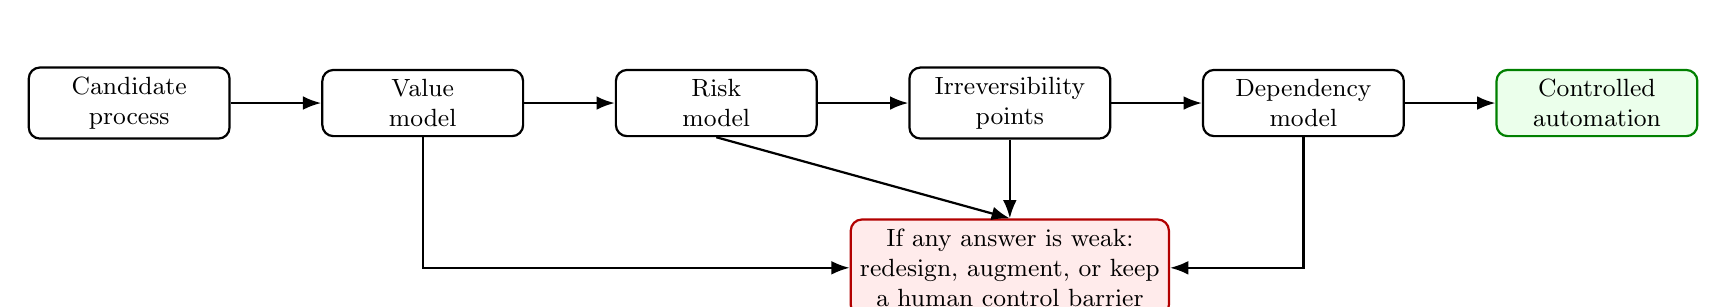
\begin{tikzpicture}[node distance=1.15cm, every node/.style={font=\small}, box/.style={rectangle, rounded corners, draw=black, thick, align=center, minimum width=2.55cm, minimum height=0.8cm}, warn/.style={rectangle, rounded corners, draw=red!70!black, thick, align=center, minimum width=2.55cm, minimum height=0.8cm, fill=red!8}, ok/.style={rectangle, rounded corners, draw=green!50!black, thick, align=center, minimum width=2.55cm, minimum height=0.8cm, fill=green!8}, arrow/.style={-{Latex}, thick}]
\node[box] (p) {Candidate\\process};
\node[box, right=of p] (v) {Value\\model};
\node[box, right=of v] (r) {Risk\\model};
\node[box, right=of r] (i) {Irreversibility\\points};
\node[box, right=of i] (d) {Dependency\\model};
\node[ok, right=of d] (a) {Controlled\\automation};
\node[warn, below=1.0cm of i] (g) {If any answer is weak:\\redesign, augment, or keep\\a human control barrier};
\draw[arrow] (p) -- (v);
\draw[arrow] (v) -- (r);
\draw[arrow] (r) -- (i);
\draw[arrow] (i) -- (d);
\draw[arrow] (d) -- (a);
\draw[arrow] (v.south) |- (g.west);
\draw[arrow] (r.south) -- (g.north);
\draw[arrow] (i.south) -- (g.north);
\draw[arrow] (d.south) |- (g.east);
\end{tikzpicture}%
}
\caption{A minimal decision framework for hyperautomation. Automation is justified only when value, risk, irreversibility, dependency, and capability are explicitly considered.}
\end{figure}

\section{Conclusion: from offshore execution to systemic innovation}
Generative AI does not make human work obsolete. It exposes the weakness of work designed as isolated fragments. The response should not be panic, nor blind automation. It should be systemic capability building.

For Latin America, the opportunity is significant. The region has engineering talent, universities, emerging startups, and examples of industrial excellence. But capturing the next wave of value requires reinvestment in applied research, product engineering, system architecture, and leadership models that grow people beyond narrow execution. Offshoring can be a source of income. It should also become a bridge toward industrialization and innovation.

For managers, the practical path is slower and more human than the hype suggests. Encourage. Accompany. Guide. Show by doing. Repeat. The objective is not to eliminate specialization, but to prevent cognitive enclosure. The future belongs less to interchangeable task executors than to connected specialists who understand the systems they help build.

\section*{Acknowledgements and note}
This memo is personal and reflective. It does not represent the official position of any employer, client, or institution. It proposes conceptual interpretations grounded in operational experience and selected literature, not a statistically validated causal model. Operational examples are illustrative composites and not descriptions of identifiable individuals, clients, production environments, or operational incidents. It is intended as a research-style appendix to a shorter LinkedIn post and as a working basis for further discussion with practitioners, researchers, and engineering leaders.

\printbibliography

\appendix
\section{Short LinkedIn teaser}
\begin{quote}
Generative AI will not kill your job. But your work design might.

We often ask the wrong question: ``Will AI replace people?'' A better one may be: what kind of work have we already made replaceable by fragmenting it into narrow, repeatable, context-blind tasks?

In secure document issuance, automation can create real value. But what happens when the system silently validates something a human might question? Not because the AI fails loudly, but because it does not hesitate.

My thesis: AI does not end work; it exposes fragmented work. And it does not just replace human error -- it can replace human hesitation. The answer is not more specialization, but systemic capability and connected specialists.
\end{quote}

\section{Conceptual glossary}
\begin{description}[leftmargin=2.8cm, style=nextline]
\item[Hyperautomation] A strategy that combines workflow automation, AI, RPA, APIs, orchestration, and data pipelines to automate increasingly complex processes.
\item[Work fragmentation] The decomposition of work into narrow tasks, roles, tickets, or service functions, often improving measurability but reducing systemic understanding.
\item[Connected specialization] Deep expertise combined with the ability to understand adjacent domains and system-level consequences.
\item[Irreversibility] The degree to which an error becomes costly, public, or impossible to correct once it crosses a process boundary.
\item[Silent false negative] An error that passes undetected because it falls outside the distribution a model was trained on or the anomaly classes it was designed to flag: no alert, no friction, no correction opportunity.
\item[Sociotechnical Systems (STS)] A design and diagnostic theory holding that effective organizations must optimize their social and technical subsystems jointly, rather than designing the technical system first and treating humans as residual components. Originating from Trist and colleagues at the Tavistock Institute (UK coal mines, 1950s), STS argues that flexibility, trust, and cognitive diversity are performance criteria as important as efficiency -- especially in innovation-intensive contexts where human adaptive capacity cannot be engineered away.
\item[Cognitive dependency] Reliance on external tools, models, platforms, or vendors not only for execution but for interpretation and decision support.
\end{description}

\end{document}
